\section{Our Approach}
\label{sec:pipelining-algorithm}

Pipeline synthesis is based on the key observation that
successive iterations can be overlapped without affecting execution as long
as data and control dependecies are correctly maintained. 
Thus, the three main
activities of a pipeline synthesis algorithm are to
(1)~identify and remove possible hazards (2)~overlap the
successive iterations according to the pipeline interval, and 
(3)~ensure proper placement of conditional and unconditional branches. In our case,
the identification of data hazards is simplified since the synthesis tool
provides a pipeline interval. If we can use this pipeline interval to build our design, 
then the pipeline reference model is comparable to RTL in abstraction. 

We have developed a framework of five certified pipelining
primitives which allows us, among other things, to prevent possible data
hazards. Our framework also provides a primitive
to overlap successive iterations and a provision to add and remove 
branches when required while still maintaining the control flow. We now discuss
the framework in detail.

\subsection{Framework of Provable Pipelining Primitives}

We believe that the following primitives are necessary and essential in creating any pipelining
algorithm in behavioral synthesis.

{\textbf {$\phi$-elimination primitive}} -- 
Reasoning about the $\phi$-statement is complex since after its
execution from a state, say $s$, the state reached depends not only
on the state $s$ but also on previous basic blocks in the execution history.
However, we must handle it since it is used extensively in
loops to perform different actions depending on whether the
loop body is executed the first time. One of the key steps in loop pipelining is,
therefore, $\phi$-elimination {\em i.e.}, replacing
$\phi$-statement with appropriate assignment statements when the previous basic block is known.

{\textbf {Shadow register primitive}} -- We define a shadow register microstep as an assignment
statement with symbol expression ($x$) assigned to a new value ($x\_reg$). We call all the new introduced 
variables as shadow registers. Intuitively, it is correct that in a sequence of steps, if we assign a variable 
to a shadow register and replace all occurences of $x$ with $x\_reg$
till the next write of $x$, we should
not have made any difference in the execution. Also, since we are not changing the value of $x$ itself, 
the state after end of execution for both CCDFGs as far as real variables are concerned (all variables
 excluding all shadow registers) is same. 

\begin{figure}[H]
\begin{center}
\begin{tabular}{cc}
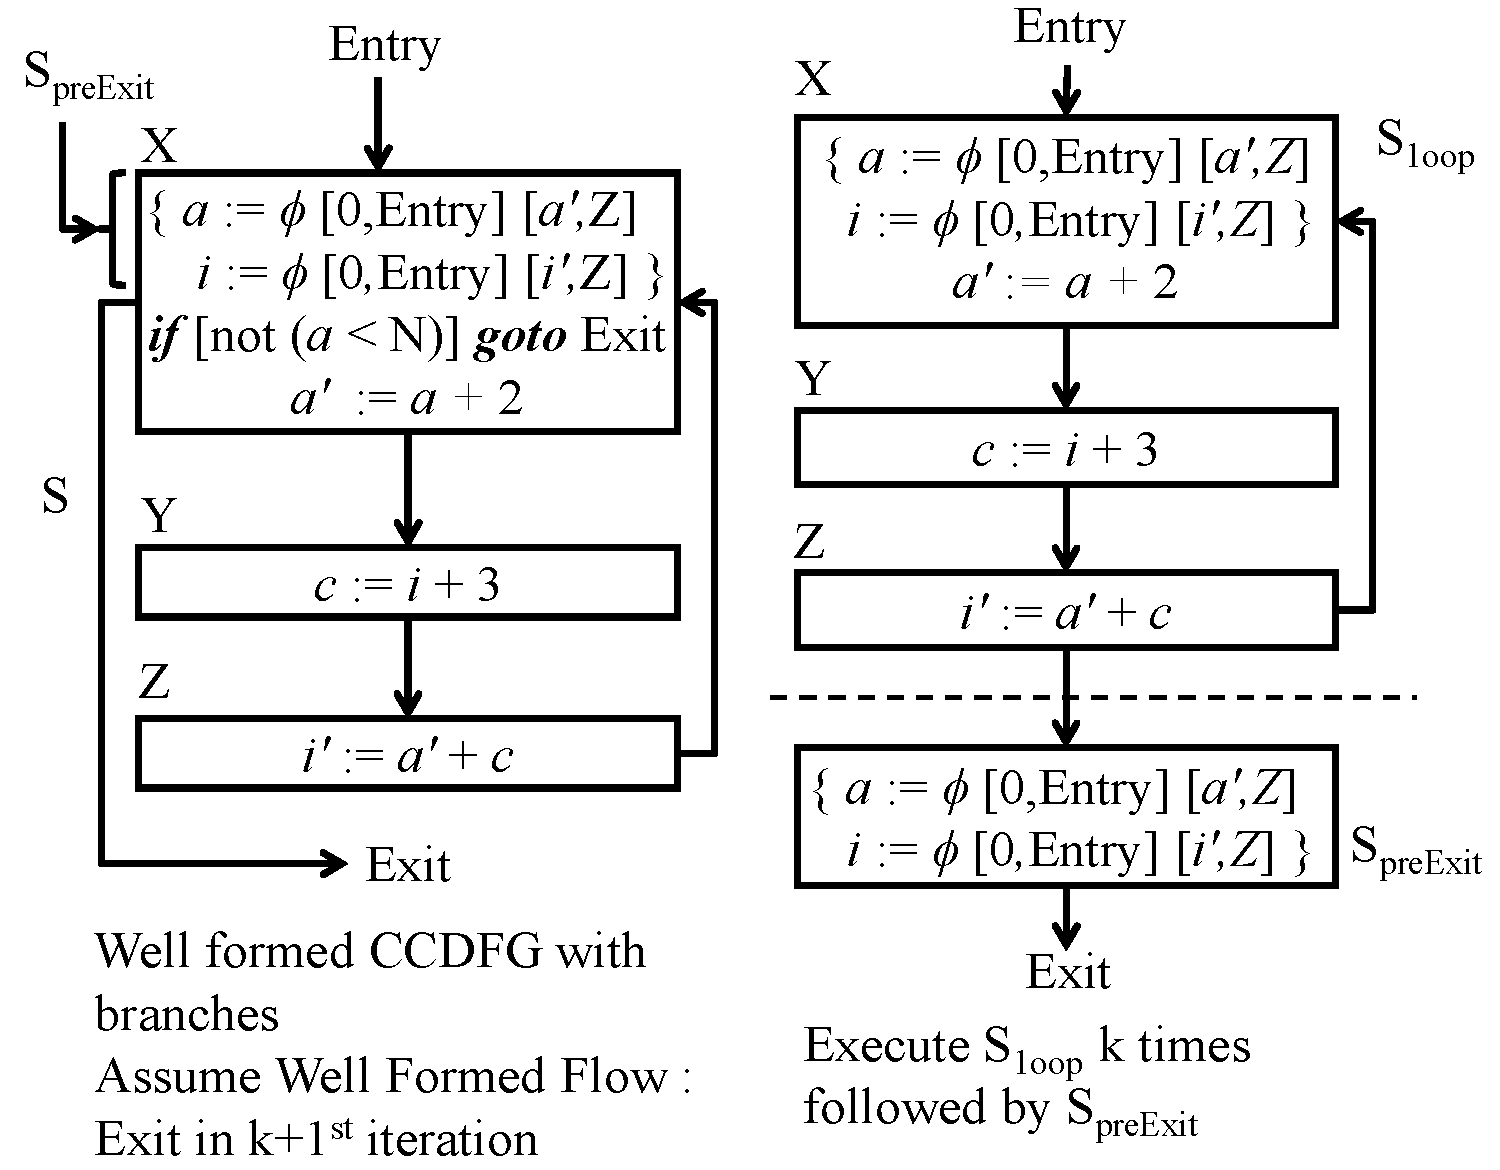
\includegraphics[height=1.8in]{fig-proposal/conditional-branch-primitive}
& 
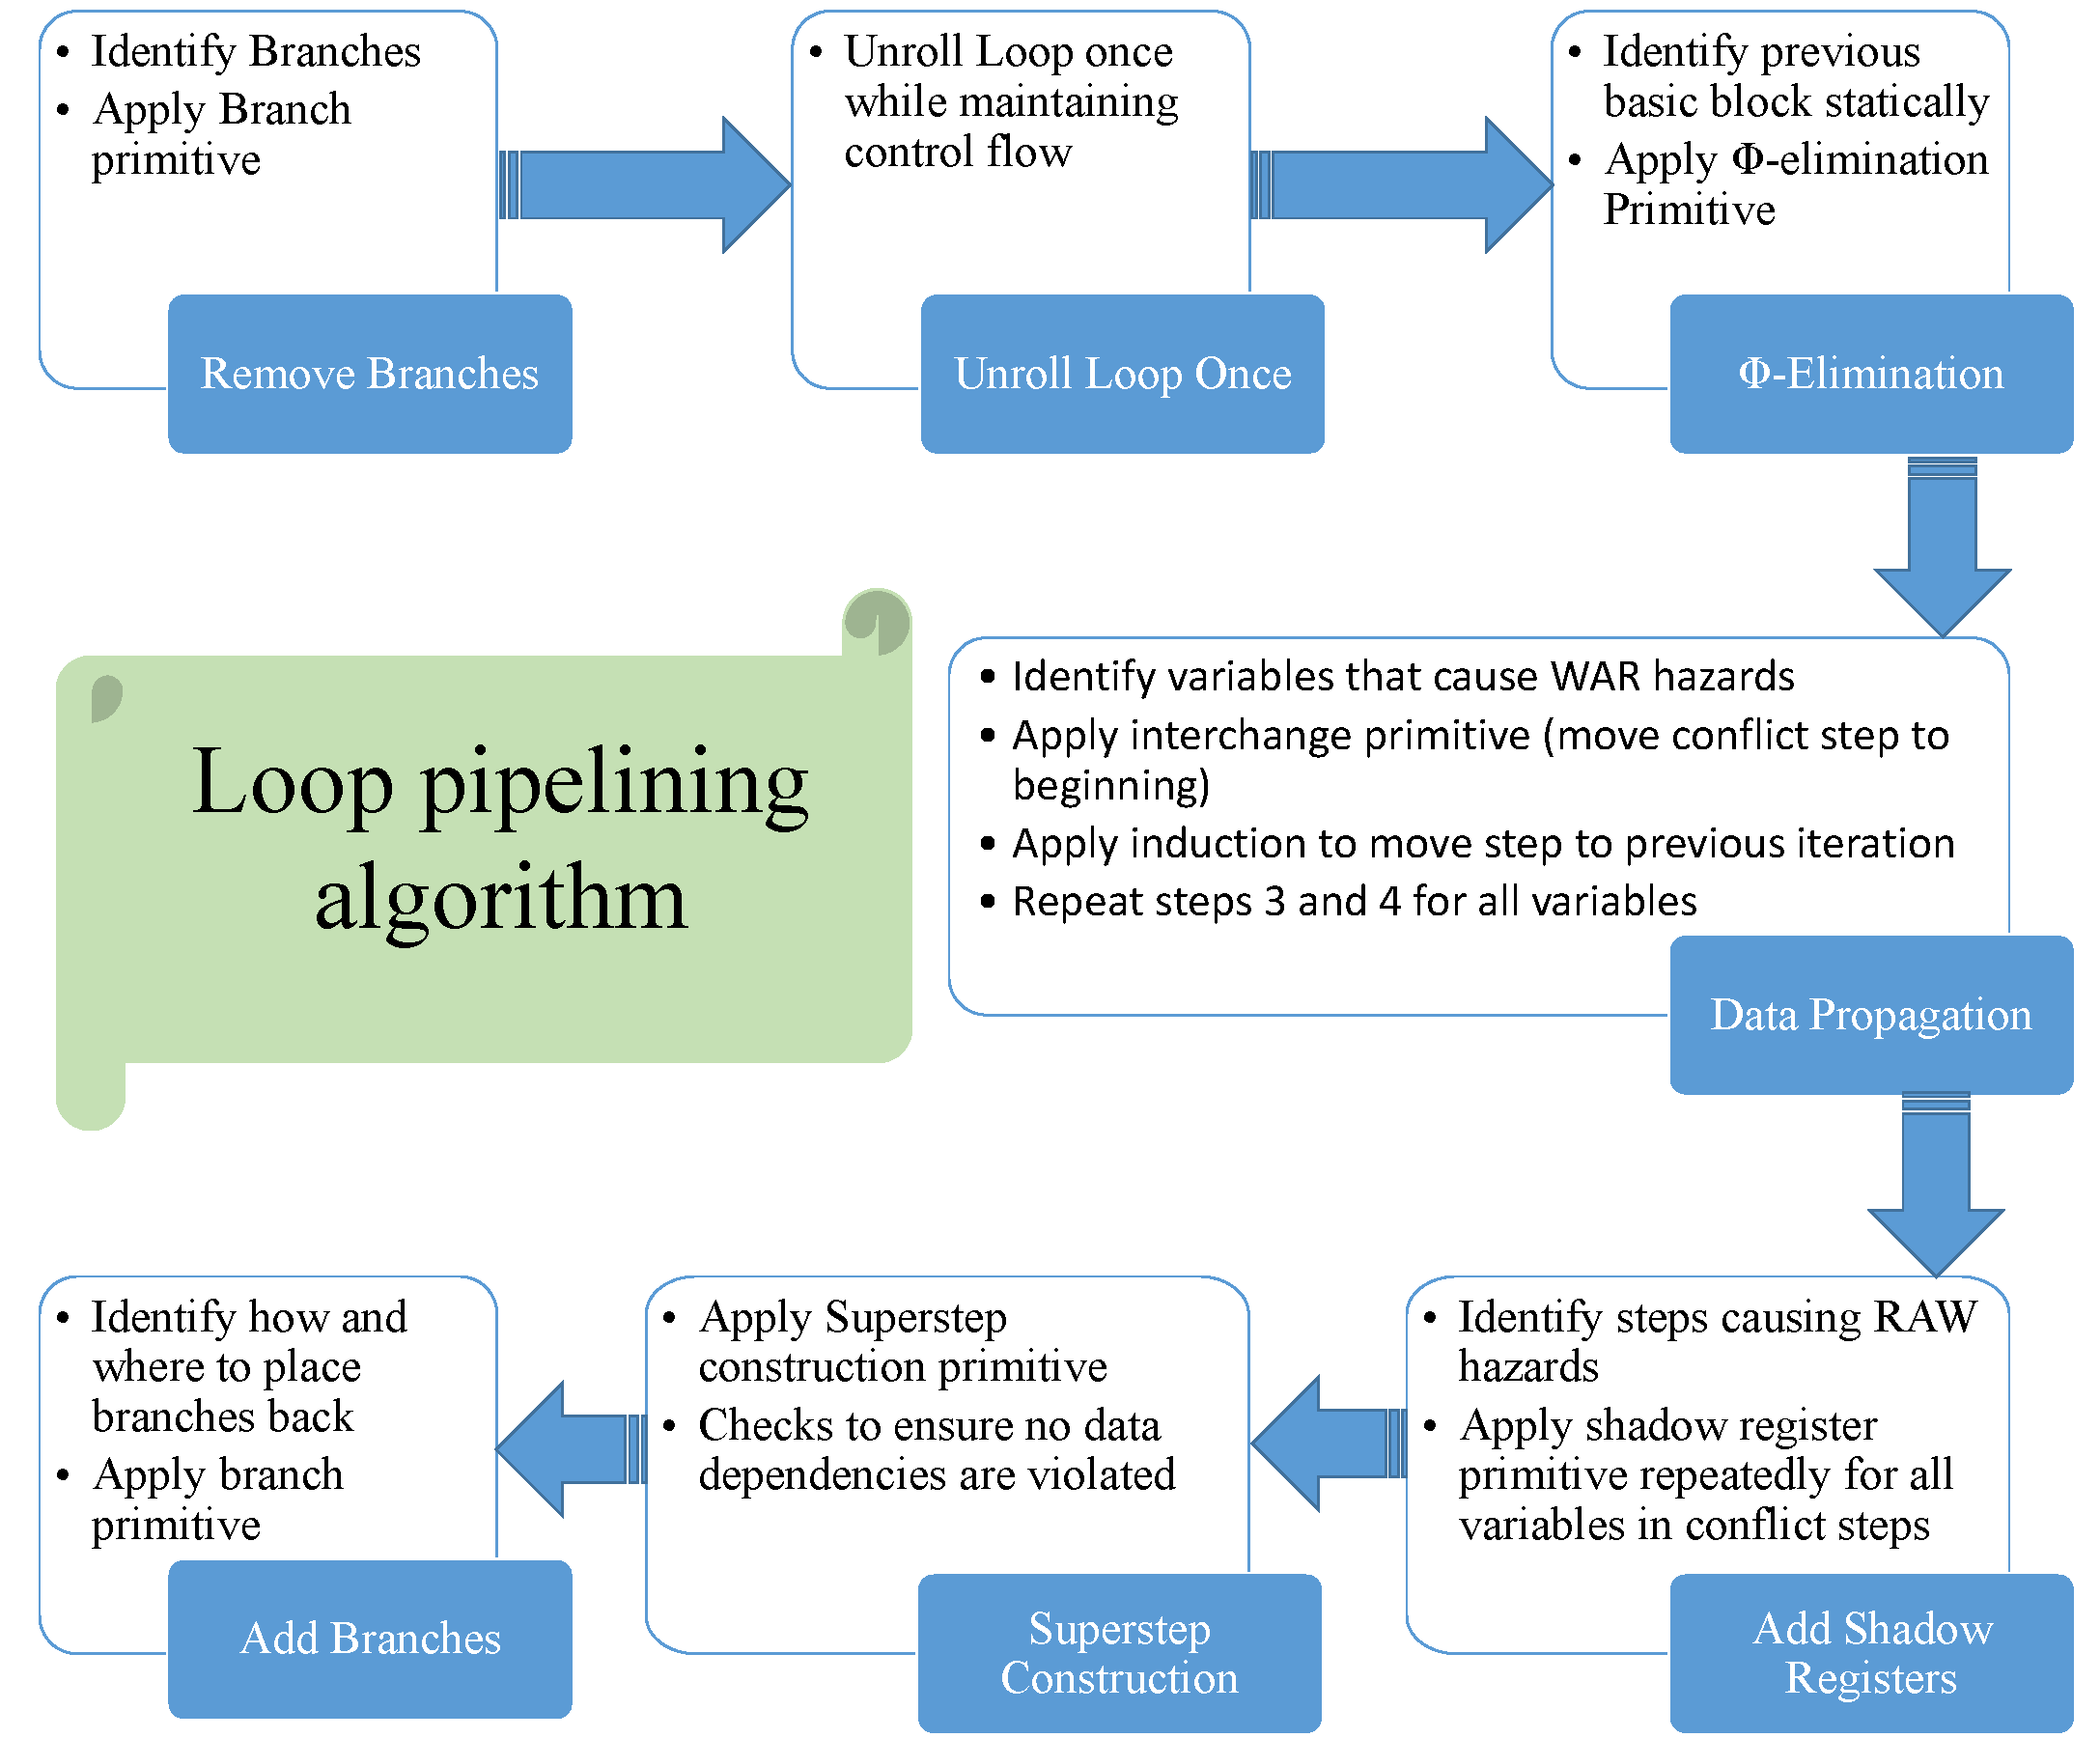
\includegraphics[height=1.8in]{fig-proposal/algorithm-using-primitives}
\\
(a) &  (b) 
\end{tabular}
\end{center}
\caption{(a) Branch Primitive (b) Algorithm Using Primitives}
\label{fig:branch-primitive}
\end{figure}

{\textbf {Branch primitive}} -- Branch instructions are required for control flow. However, reasoning about 
execution of branch instructions in a loop everytime we apply a primitive can make proof very complex.
We note that if we specifically assume that the exit condition becomes true after completing $k$ iterations, then we can remove the conditional branch.
To understand the branch primitive (c.f. Figure~\ref{fig:branch-primitive}), 
let's assume there is a conditional branch in the sequential loop structure $S$, which points to either
the next microstep in sequence or exits the loop by branching to the scheduling step
$Exit$. Let $S_{preExit}$ be the collection of microsteps before this branch in $S$ and
let $S_{loop}$ be the corresponding CCDFG loop without the conditional branch.
The conditional branch primitive allows us to replace $S$ with $S_{loop}$ followed by
$S_{preExit}$. Similarly,
the primitive also allows us to introduce an exit conditional branch by replacing
$S_{loop}$ followed by $S_{preExit}$ with $S$.
Note that since $k$ can take any value $k \ge 0$, we are not compromising on the correctness statement.  
It can be proved that executing $S$ such that it exits in the $(k+1)$ st
iteration is same as executing $S_{loop}$ $k$ times followed by $S_{preExit}$.

{\textbf {Interchange primitive}} -- Let $m$ and $n$ be two adjacent scheduling steps (or collection of microsteps) in a CCDFG where both $m$ and $n$ do not have read hazards and any microsteps containing branch statements. Then, the interchange primitive allows us to interchange their order without affecting execution. 

{\textbf {Superstep construction primitive}} -- This entails combining the scheduling steps of the successive
iterations, forming scheduling ``supersteps'' that act as scheduling steps for the pipelined implementation. Supersteps must
account for read-after-write hazards, i.e, if a variable is written in a scheduling step $X$ and read subsequently in
$Z$ then $Z$ cannot be in a superstep that precedes $X$ in the control/data flow.  Note that we implement data
forwarding (forward value of data within a single clock cycle); thus $X$ and $Z$ can be in a single superstep.

\subsection{Our Loop Pipelining Algorithm}

Given a sequential loop $S$ in CCDFG $C$ and pipeline interval $I$, we can create a pipelined loop $P$ using Algorithm~\ref{algo:loop}. Note that every step of the algorithm is build from ground up using our framework of provable primitives such that the algorithm can be certified by theorem proving (c.f. Figure~\ref{fig:branch-primitive} (b)). 

\begin{algorithm}[H]
\caption{Pipelining Algorithm}
\label{algo:loop}
\begin{algorithmic}[1]
\Procedure{PipelineLoop}{S, I}
\State $S_1 \leftarrow RemoveBranches(S)$
\State $S_2 \leftarrow UnrollLoopOnce(S_1)$
\State $S_3 \leftarrow \phi-Elimination (S_2) $.
\State $S_4 \leftarrow DataPropagation (S_3, I) $.
\State $S_5 \leftarrow GenerateShadowRegisters (S_4, I) $.
\State $ S_6 \leftarrow SuperstepConstruction (S_5, I) $.
\State $P \leftarrow AddBranches (S_6) $
\State \textbf{return} $(P)$.
\EndProcedure
\end{algorithmic}
\end{algorithm}

Now, we describe the steps to convert a sequential loop CCDFG $S$ (c.f. Figure~\ref{fig:branch-primitive}) to a pipelined loop CCDFG:

{\bf Remove Branches}: We apply the branch primitive on $S$ to remove branches by explicitly defining the control flow. 

{\bf Unroll Loop Once}: The first iteration behaves differently than the rest due to $\phi$-construct. So, we unroll the loop $S_{loop}$ once and call it $S_{pre}$. 

{\bf $\phi$-elimination}: We apply the $\phi$-elimination primitive on $S_{pre}$, $S_{loop}$ and $S_{preExit}$ to return a CCDFG in which all the $\phi$-statements have been replaced with their corresponding assignment statements. 

\begin{algorithm}
\caption{Data propagation} 
\label{algo:data-propagation}
\begin{algorithmic}[1]
\Procedure{DataPropogration}{$L$}
\State $msteps \leftarrow GetLoopCarriedDependencies(L)$
\For {\textbf{each} mstep \textbf{in} msteps}
\If {$CheckConflict (L, mstep, N, I) \neq 0$}
\State $L \leftarrow RelocateMStep (L, mstep)$
\EndIf
\EndFor
\State \textbf{return} $(L)$
\EndProcedure
\end{algorithmic}
\end{algorithm}

{\bf Data propagation:} Algorithm~\ref{algo:data-propagation} describes how to compute candidates for data
propagation across pipeline iterations. It is a critical step as we want to make sure that when we pipeline a loop, we do not read a variable which has not
yet been written. A critical observation is that data propagation is required only for loop carried dependencies.
$GetLoopCarriedDependencies$ identifies the microsteps where loop carried dependencies are being read. Then,
$CheckConflict$ checks whether there would be a conflict when we pipeline the loop. Conflict occurs when the value being read in a microstep is not yet written in the pipelined loop execution. If so, $RelocateMSteps$ relocates the microstep which is causing the data hazard to the previous iteraton. Note that this step requires multiple applications of interchange primitive and very complex induction. This step ensures that any variable which is being read has already been written. Note that in order to maintain the invariant, only those microsteps can be propagated which exist in $S_{preExit}$, which means only those steps which occur before the conditional branch in original CCDFG can be relocated. This ensures that our algorithm does not have the bug which the previously proposed algorithm had. In Figure~\ref{fig:algo1-3}(b) we found that the loop carried dependency $i'$ in $X$ would create a conflict when we would move $X$ before $Z$ while pipelining. So, we relocate the microstep $i := i'$ as shown in Figure~\ref{fig:algo2-2}(a). This step needs to be repeated for every variable found using $GetLoopCarriedDependencies$.

\begin{figure}[t!]
\begin{center}
\begin{tabular}{cc}
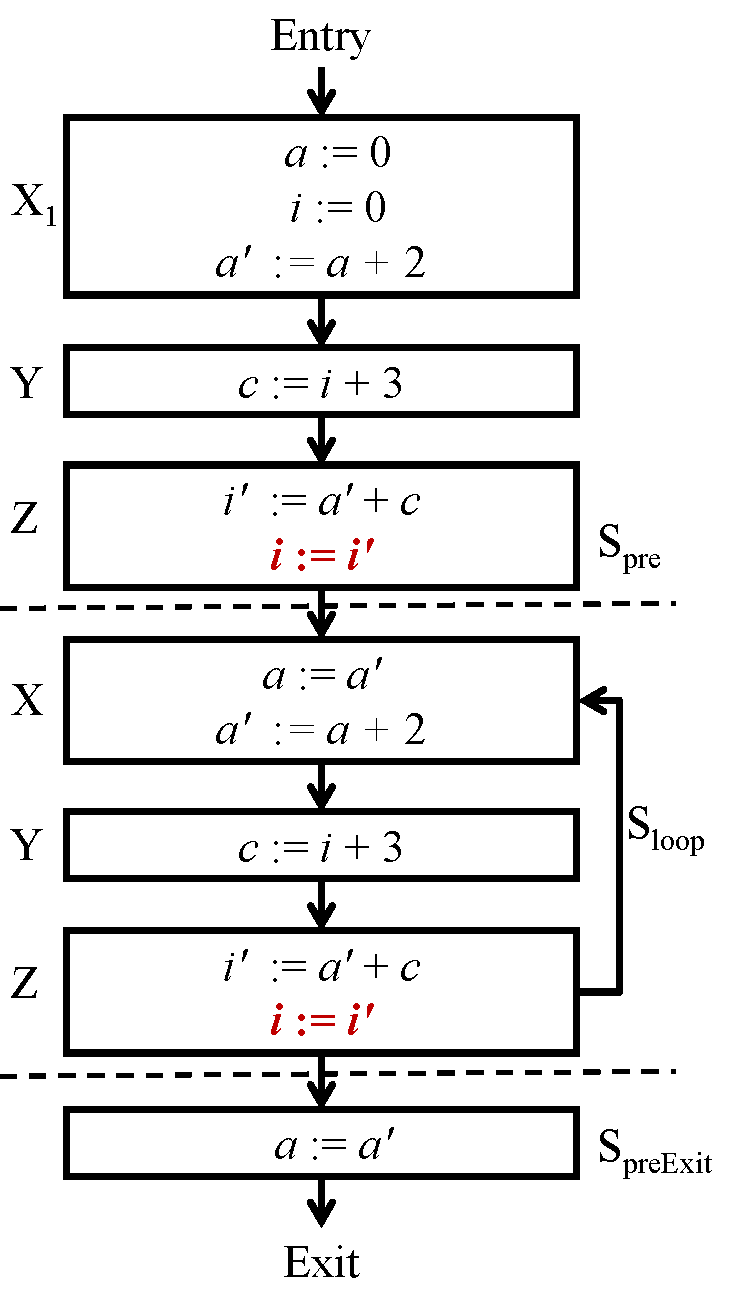
\includegraphics[height=2.5in]{fig-proposal/algorithm-after-data-propagation-2}
&
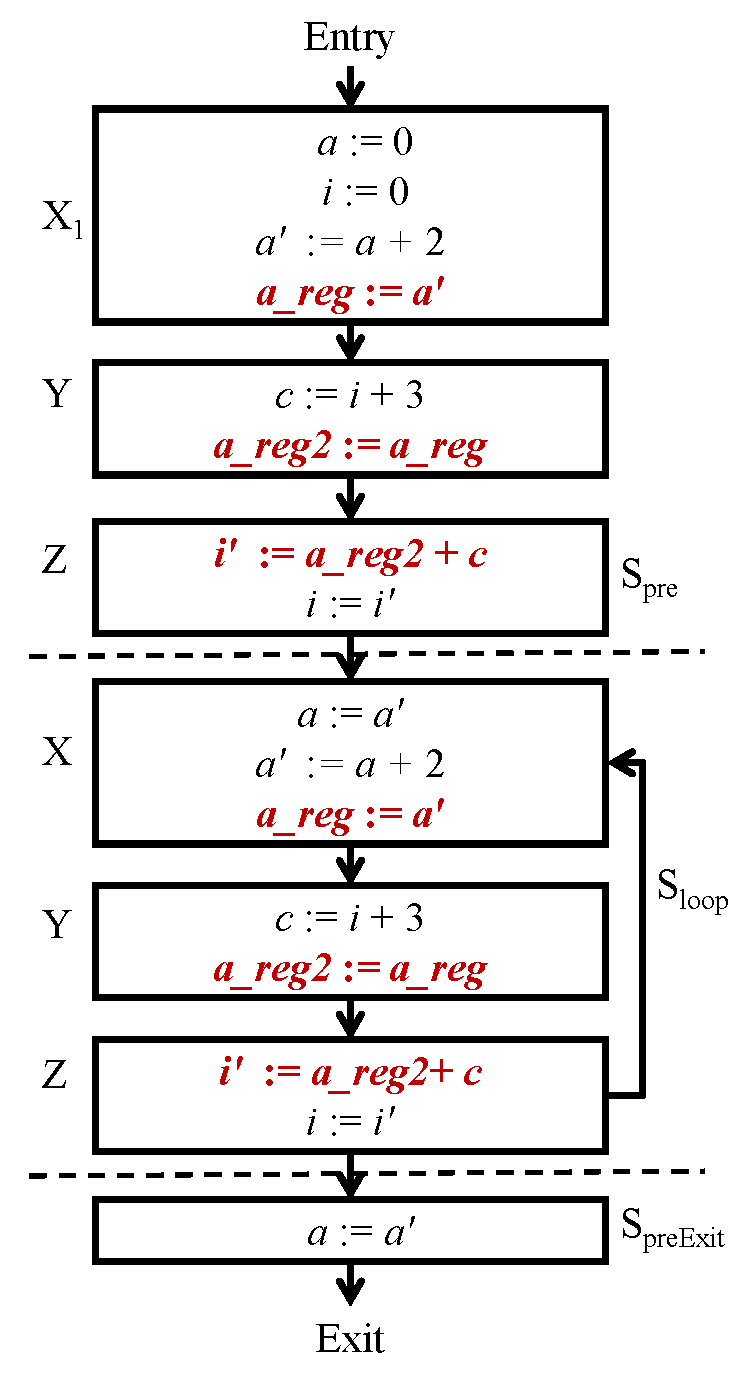
\includegraphics[height=2.5in]{fig-proposal/algorithm-after-shadow-register}
\\
(a) & (b)
\\
\end{tabular}
\end{center}
\caption{(a) After Data Propagation (b) After adding Shadow Register}
\label{fig:algo2-2}
\end{figure}

{\bf Generate shadow registers:} Algorithm~\ref{algo:generate-pipeline-registers} inserts shadow registers
to prevent variables from being overwritten before being read. We first compute all program variables that may be
overwritten before being read, which means these are the variables that require shadow registers. To find such variables,
 $GetAllVariables$ first gets a set of all variables. Then, for each variable, we compare the distance (the number of scheduling steps) between the write of
  the variable $w_v$ $(WriteVariable)$ and the last read of the variable $r_v$ $(LastReadVariable)$ in an iteration; if the
   distance is greater than $I$ (pipeline interval), the variable is assigned the new data value of the next iteration before the current iteration's value
    has been fully consumed; this warrants insertion of shadow registers in every scheduling step between the $r_v$ and $w_v$. The value is propagated every clock cycle following the CCDFG data flow. In Figure~\ref{fig:algo2-2}(b), we introduce a shadow register $a\_reg$ in $X$ and $a\_reg2$ in $Y$. This step is also repeated for all the variables found using $GetAllVariables$.

\begin{algorithm}[H]
\caption{Generate shadow registers} 
\label{algo:generate-pipeline-registers}
\begin{algorithmic}[1]
\Procedure{GenerateShadowRegisters}{$L$, $I$}
\State $V \leftarrow GetAllVariables(L)$.
\For {\textbf{each} v \textbf{in} V}
\State $w_v \leftarrow WriteVariable (v, L)$.
\State $r_v \leftarrow LastReadVariable (v, L)$.
\If {$RequireShadowRegister (r_v, w_v, I) \neq 0$}
\State $L \leftarrow AddShadowRegister (w_v, L)$.
\EndIf
\EndFor
\State \textbf{return} $(L)$.
\EndProcedure
\end{algorithmic}
\end{algorithm}



\begin{figure}[t!]
\begin{center}
\begin{tabular}{cc}
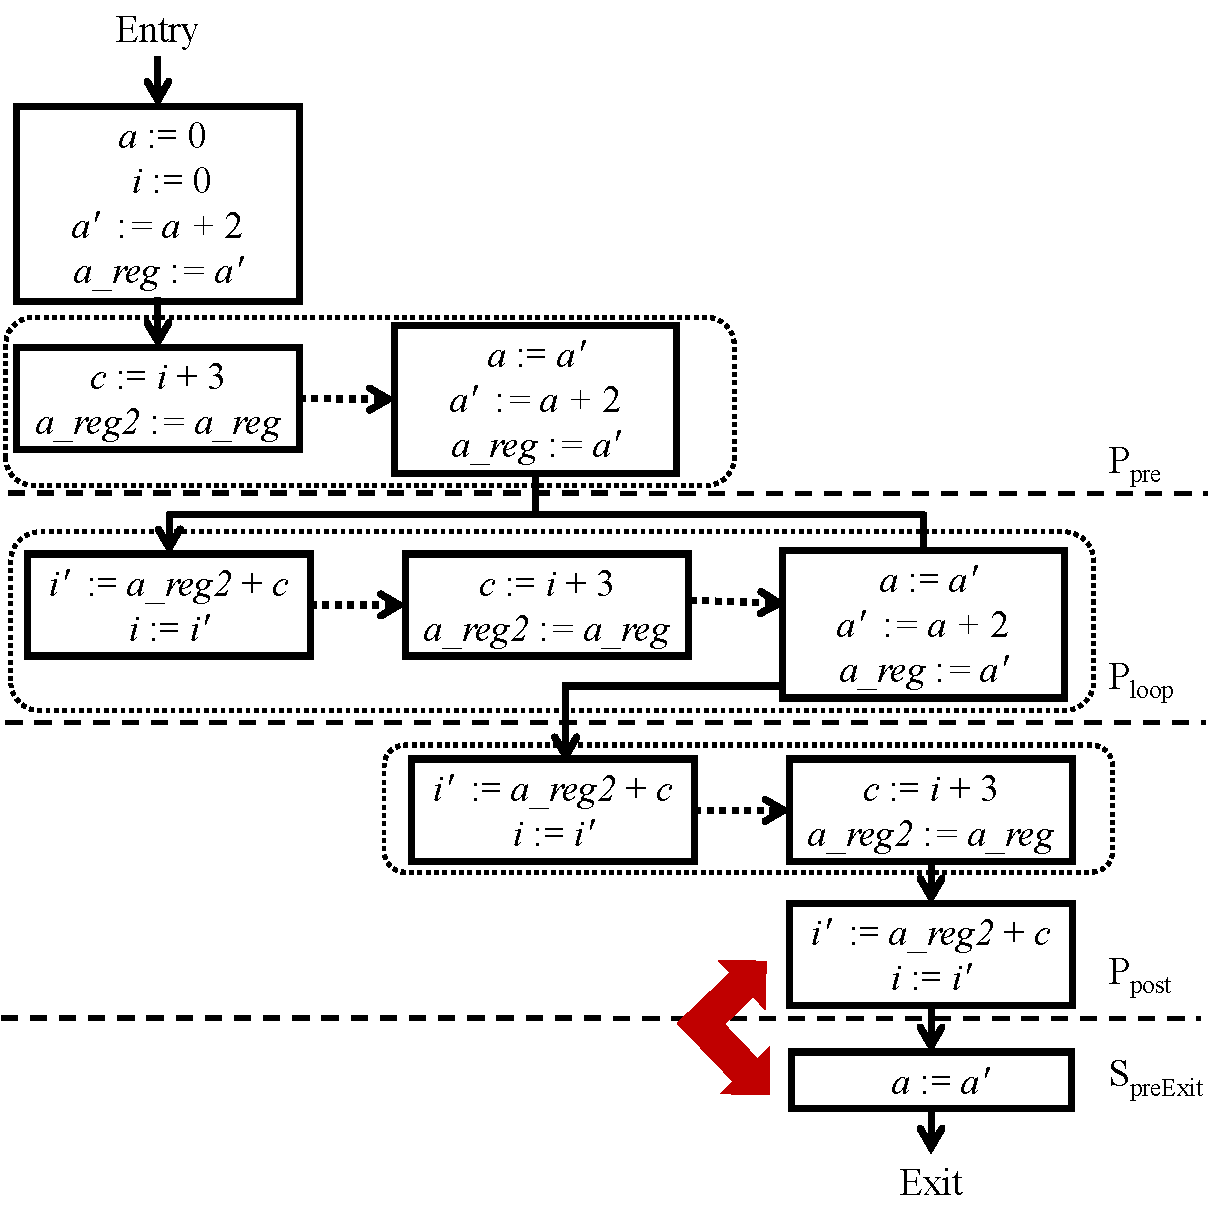
\includegraphics[height=2in]{fig-proposal/algorithm-after-superstep-construction}
&
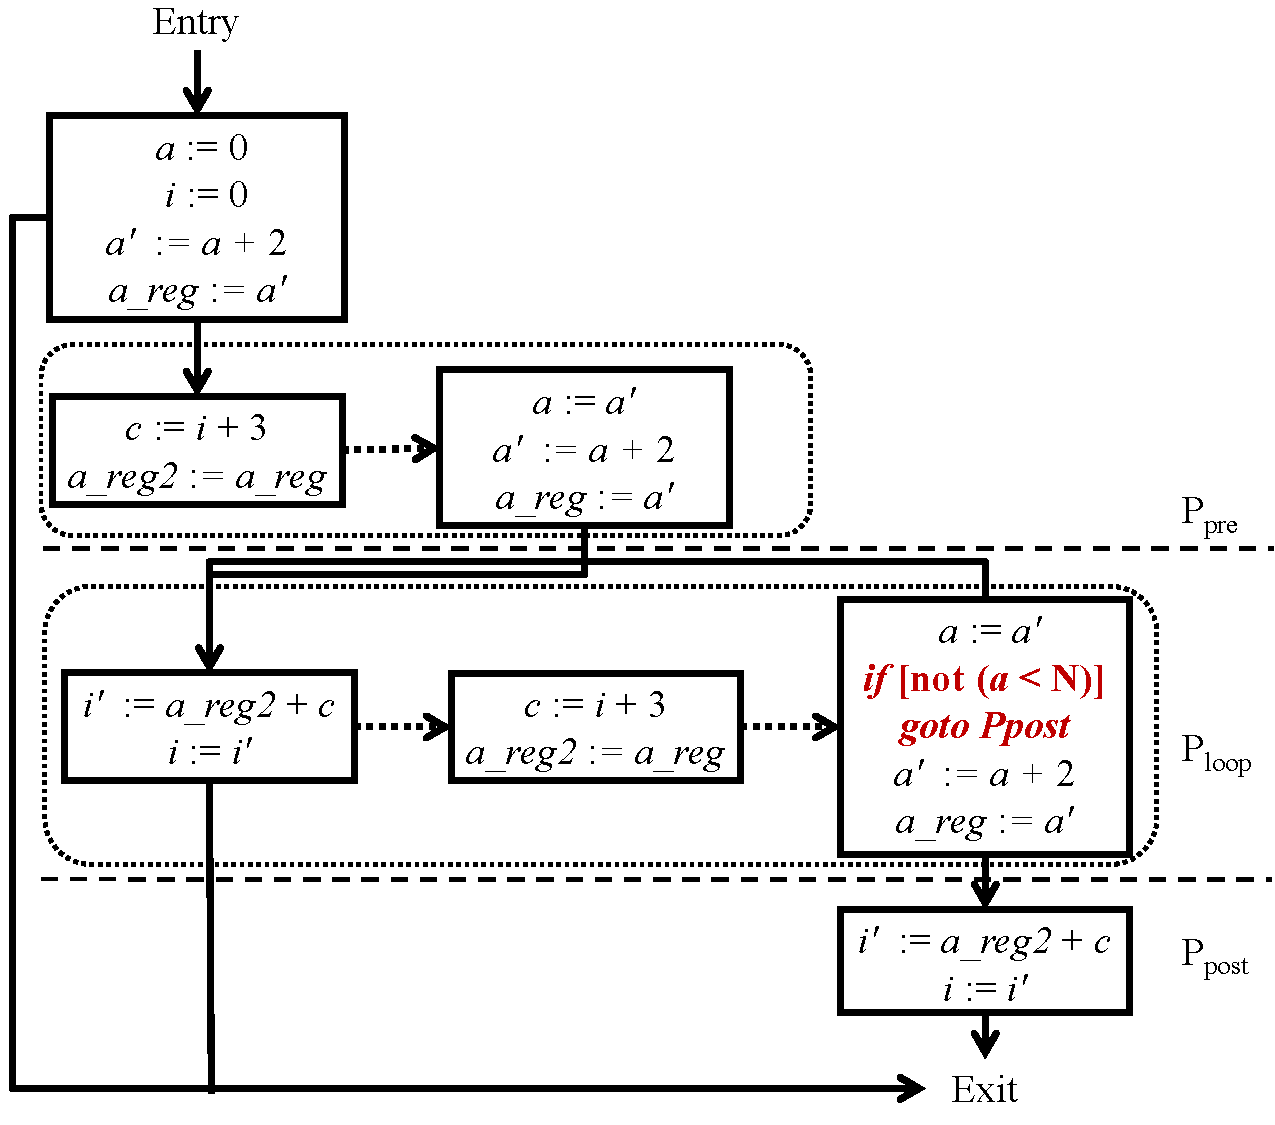
\includegraphics[height=2in]{fig-proposal/algorithm-after-adding-branches}
\\
(a) & (b)
\\
\end{tabular}
\end{center}
\caption{(a) After superstep construction (b) Final Pipelined CCDFG}
\label{fig:algo3-2}
\end{figure}

{\bf Superstep construction:} Now that we have removed the data hazards, we can successfully pipeline the loop using  the pipeline interval $I$. We combine the scheduling steps of the successive iterations, forming scheduling ``supersteps'' that act as scheduling steps for the pipelined
implementation. A scheduling step is allowed to move up another scheduling step only if there are no intermediate read and write conflicts. Note that we implement data forwarding; thus $s$ and $s'$ can be in a single scheduling superstep.
Superstep construction on $S_{pre}$ and $S_{loop}$ creates a CCDFG with three parts: prologue $P_{pre}$, $P_{loop}$ which is the full pipeline stage and epilogue $P_{post}$ as shown in Figure~\ref{fig:algo3-2}. 

{\bf Add Branches:}  To add the branches back, we use the a combination of interchange primitive and reverse of Branch primitive. Note in Figure~\ref{fig:algo3-2}, if there are no read write hazards in between the last scheduling step $Z$ of $P_{post}$ and $S_{preExit}$, we can interchange them using interchange primtive. Now recall from the branch primitive that if there is a loop structure $S_{loop}$ with a conditional branch, then executing $S_{loop}$ such that it exits in the (k+1)st iteration is same as executing $S_{loop}$ without the conditional branch followed by only those steps from $S_{loop}$ which occur before the branch $S_{preExit}$. Now, we apply the reverse of branch primitive here. $P_{loop}$ in Figure~\ref{fig:algo3-2} is a loop structure without a conditional branch, followed by a collection of microsteps $P_{preExit}$ (here, a collection of $Z$, $Y$ and $S_{preExit}$). Then, we can add an exit conditional branch in $P_{loop}$ after the microsteps $P_{preExit}$. This branch points to the next scheduling step after the loop $P_{post}$ if the exit condition is true. We can add the conditional and the unconditional branch as shown in  Figure~\ref{fig:algo3-2}(b).  

We now have the final pipelined loop structure. We describe a proof sketch for the primitives and the algorithm in the next section.
